\documentclass[ignorenonframetext,]{beamer}
\setbeamertemplate{caption}[numbered]
\setbeamertemplate{caption label separator}{: }
\setbeamercolor{caption name}{fg=normal text.fg}
\beamertemplatenavigationsymbolsempty
\usepackage{lmodern}
\usepackage{amssymb,amsmath}
\usepackage{ifxetex,ifluatex}
\usepackage{fixltx2e} % provides \textsubscript
\ifnum 0\ifxetex 1\fi\ifluatex 1\fi=0 % if pdftex
  \usepackage[T1]{fontenc}
  \usepackage[utf8]{inputenc}
\else % if luatex or xelatex
  \ifxetex
    \usepackage{mathspec}
  \else
    \usepackage{fontspec}
  \fi
  \defaultfontfeatures{Ligatures=TeX,Scale=MatchLowercase}
\fi
\usetheme{AnnArbor}
\usecolortheme{dolphin}
\usefonttheme{professionalfonts}
% use upquote if available, for straight quotes in verbatim environments
\IfFileExists{upquote.sty}{\usepackage{upquote}}{}
% use microtype if available
\IfFileExists{microtype.sty}{%
\usepackage{microtype}
\UseMicrotypeSet[protrusion]{basicmath} % disable protrusion for tt fonts
}{}
\newif\ifbibliography
\usepackage{color}
\usepackage{fancyvrb}
\newcommand{\VerbBar}{|}
\newcommand{\VERB}{\Verb[commandchars=\\\{\}]}
\DefineVerbatimEnvironment{Highlighting}{Verbatim}{commandchars=\\\{\}}
% Add ',fontsize=\small' for more characters per line
\usepackage{framed}
\definecolor{shadecolor}{RGB}{248,248,248}
\newenvironment{Shaded}{\begin{snugshade}}{\end{snugshade}}
\newcommand{\KeywordTok}[1]{\textcolor[rgb]{0.13,0.29,0.53}{\textbf{{#1}}}}
\newcommand{\DataTypeTok}[1]{\textcolor[rgb]{0.13,0.29,0.53}{{#1}}}
\newcommand{\DecValTok}[1]{\textcolor[rgb]{0.00,0.00,0.81}{{#1}}}
\newcommand{\BaseNTok}[1]{\textcolor[rgb]{0.00,0.00,0.81}{{#1}}}
\newcommand{\FloatTok}[1]{\textcolor[rgb]{0.00,0.00,0.81}{{#1}}}
\newcommand{\ConstantTok}[1]{\textcolor[rgb]{0.00,0.00,0.00}{{#1}}}
\newcommand{\CharTok}[1]{\textcolor[rgb]{0.31,0.60,0.02}{{#1}}}
\newcommand{\SpecialCharTok}[1]{\textcolor[rgb]{0.00,0.00,0.00}{{#1}}}
\newcommand{\StringTok}[1]{\textcolor[rgb]{0.31,0.60,0.02}{{#1}}}
\newcommand{\VerbatimStringTok}[1]{\textcolor[rgb]{0.31,0.60,0.02}{{#1}}}
\newcommand{\SpecialStringTok}[1]{\textcolor[rgb]{0.31,0.60,0.02}{{#1}}}
\newcommand{\ImportTok}[1]{{#1}}
\newcommand{\CommentTok}[1]{\textcolor[rgb]{0.56,0.35,0.01}{\textit{{#1}}}}
\newcommand{\DocumentationTok}[1]{\textcolor[rgb]{0.56,0.35,0.01}{\textbf{\textit{{#1}}}}}
\newcommand{\AnnotationTok}[1]{\textcolor[rgb]{0.56,0.35,0.01}{\textbf{\textit{{#1}}}}}
\newcommand{\CommentVarTok}[1]{\textcolor[rgb]{0.56,0.35,0.01}{\textbf{\textit{{#1}}}}}
\newcommand{\OtherTok}[1]{\textcolor[rgb]{0.56,0.35,0.01}{{#1}}}
\newcommand{\FunctionTok}[1]{\textcolor[rgb]{0.00,0.00,0.00}{{#1}}}
\newcommand{\VariableTok}[1]{\textcolor[rgb]{0.00,0.00,0.00}{{#1}}}
\newcommand{\ControlFlowTok}[1]{\textcolor[rgb]{0.13,0.29,0.53}{\textbf{{#1}}}}
\newcommand{\OperatorTok}[1]{\textcolor[rgb]{0.81,0.36,0.00}{\textbf{{#1}}}}
\newcommand{\BuiltInTok}[1]{{#1}}
\newcommand{\ExtensionTok}[1]{{#1}}
\newcommand{\PreprocessorTok}[1]{\textcolor[rgb]{0.56,0.35,0.01}{\textit{{#1}}}}
\newcommand{\AttributeTok}[1]{\textcolor[rgb]{0.77,0.63,0.00}{{#1}}}
\newcommand{\RegionMarkerTok}[1]{{#1}}
\newcommand{\InformationTok}[1]{\textcolor[rgb]{0.56,0.35,0.01}{\textbf{\textit{{#1}}}}}
\newcommand{\WarningTok}[1]{\textcolor[rgb]{0.56,0.35,0.01}{\textbf{\textit{{#1}}}}}
\newcommand{\AlertTok}[1]{\textcolor[rgb]{0.94,0.16,0.16}{{#1}}}
\newcommand{\ErrorTok}[1]{\textcolor[rgb]{0.64,0.00,0.00}{\textbf{{#1}}}}
\newcommand{\NormalTok}[1]{{#1}}
\usepackage{longtable,booktabs}
\usepackage{caption}
% These lines are needed to make table captions work with longtable:
\makeatletter
\def\fnum@table{\tablename~\thetable}
\makeatother
\usepackage{graphicx,grffile}
\makeatletter
\def\maxwidth{\ifdim\Gin@nat@width>\linewidth\linewidth\else\Gin@nat@width\fi}
\def\maxheight{\ifdim\Gin@nat@height>\textheight0.8\textheight\else\Gin@nat@height\fi}
\makeatother
% Scale images if necessary, so that they will not overflow the page
% margins by default, and it is still possible to overwrite the defaults
% using explicit options in \includegraphics[width, height, ...]{}
\setkeys{Gin}{width=\maxwidth,height=\maxheight,keepaspectratio}

% Prevent slide breaks in the middle of a paragraph:
\widowpenalties 1 10000
\raggedbottom

\AtBeginPart{
  \let\insertpartnumber\relax
  \let\partname\relax
  \frame{\partpage}
}
\AtBeginSection{
  \ifbibliography
  \else
    \let\insertsectionnumber\relax
    \let\sectionname\relax
    \frame{\sectionpage}
  \fi
}
\AtBeginSubsection{
  \let\insertsubsectionnumber\relax
  \let\subsectionname\relax
  \frame{\subsectionpage}
}

\setlength{\emergencystretch}{3em}  % prevent overfull lines
\providecommand{\tightlist}{%
  \setlength{\itemsep}{0pt}\setlength{\parskip}{0pt}}
\setcounter{secnumdepth}{0}


% \pgfdeclareimage[width=1cm]{logo}{./figures/monkeyTypewriter.png}
%\logo{\pgfuseimage{logo}}

\institute{University of Virginia}
\definecolor{links}{RGB}{42, 27, 129}
\definecolor{mypink2}{RGB}{219, 48, 122}
%\hypersetup{colorlinks,linkcolor=links,urlcolor=mypink2}
\usefonttheme{professionalfonts}

% \setbeamerfont{note page}{family*=pplx,size=\footnotesize} % Palatino for notes

\setbeamerfont{subtitle}{size=\small}

\definecolor{uvablue}{RGB}{0,85,150}
\definecolor{uvalibraryorange}{RGB}{252,175,23}
\definecolor{uvacream}{RGB}{241,229,199}
\definecolor{uvalightblue}{RGB}{163,220,230}

\setbeamercolor{block body}{bg=green,fg=green}
\setbeamercolor{block body alerted}{bg=green,fg=green}
\setbeamercolor{block body example}{bg=green,fg=green}

\setbeamercolor{caption name}{fg=uvablue}

\setbeamercolor{headline}{fg=uvacream,bg=uvacream}
\setbeamercolor{section}{fg=uvalibraryorange,bg=uvablue}
\setbeamercolor{frametitle}{fg=uvalibraryorange,bg=uvablue}
\setbeamercolor{palette primary}{bg=uvalibraryorange,fg=uvablue}
\setbeamercolor{palette secondary}{bg=uvablue,fg=uvablue}
\setbeamercolor{palette tertiary}{bg=uvalibraryorange,fg=uvablue}
\setbeamercolor{palette quarternary}{fg=uvalibraryorange,bg=uvablue}
\setbeamercolor{palette sidebar primary}{bg=uvalibraryorange,fg=uvablue}
\setbeamercolor{palette sidebar secondary}{fg=uvablue,bg=uvablue}
\setbeamercolor{palette sidebar tertiary}{fg=uvalibraryorange,bg=uvablue}
\setbeamercolor{palette sidebar quarternary}{fg=uvalibraryorange,bg=uvablue}
\setbeamercolor{structure}{bg=uvablue}



\useinnertheme{rectangles}

\titlegraphic{\vspace{-7.5mm}\includegraphics[width=0.45\paperwidth]{./figures/monkeyTypewriter.png}}

\title{``Dr.~Tustison (UVA) presentation''}
\author{Nick Tustison}
\date{}

\begin{document}
\frame{\titlepage}

\section{Developers and
collaborators}\label{developers-and-collaborators}

\begin{frame}{Founders: Brian and Nick}

\includegraphics{./figures/brian_and_nick.png}

\end{frame}

\begin{frame}

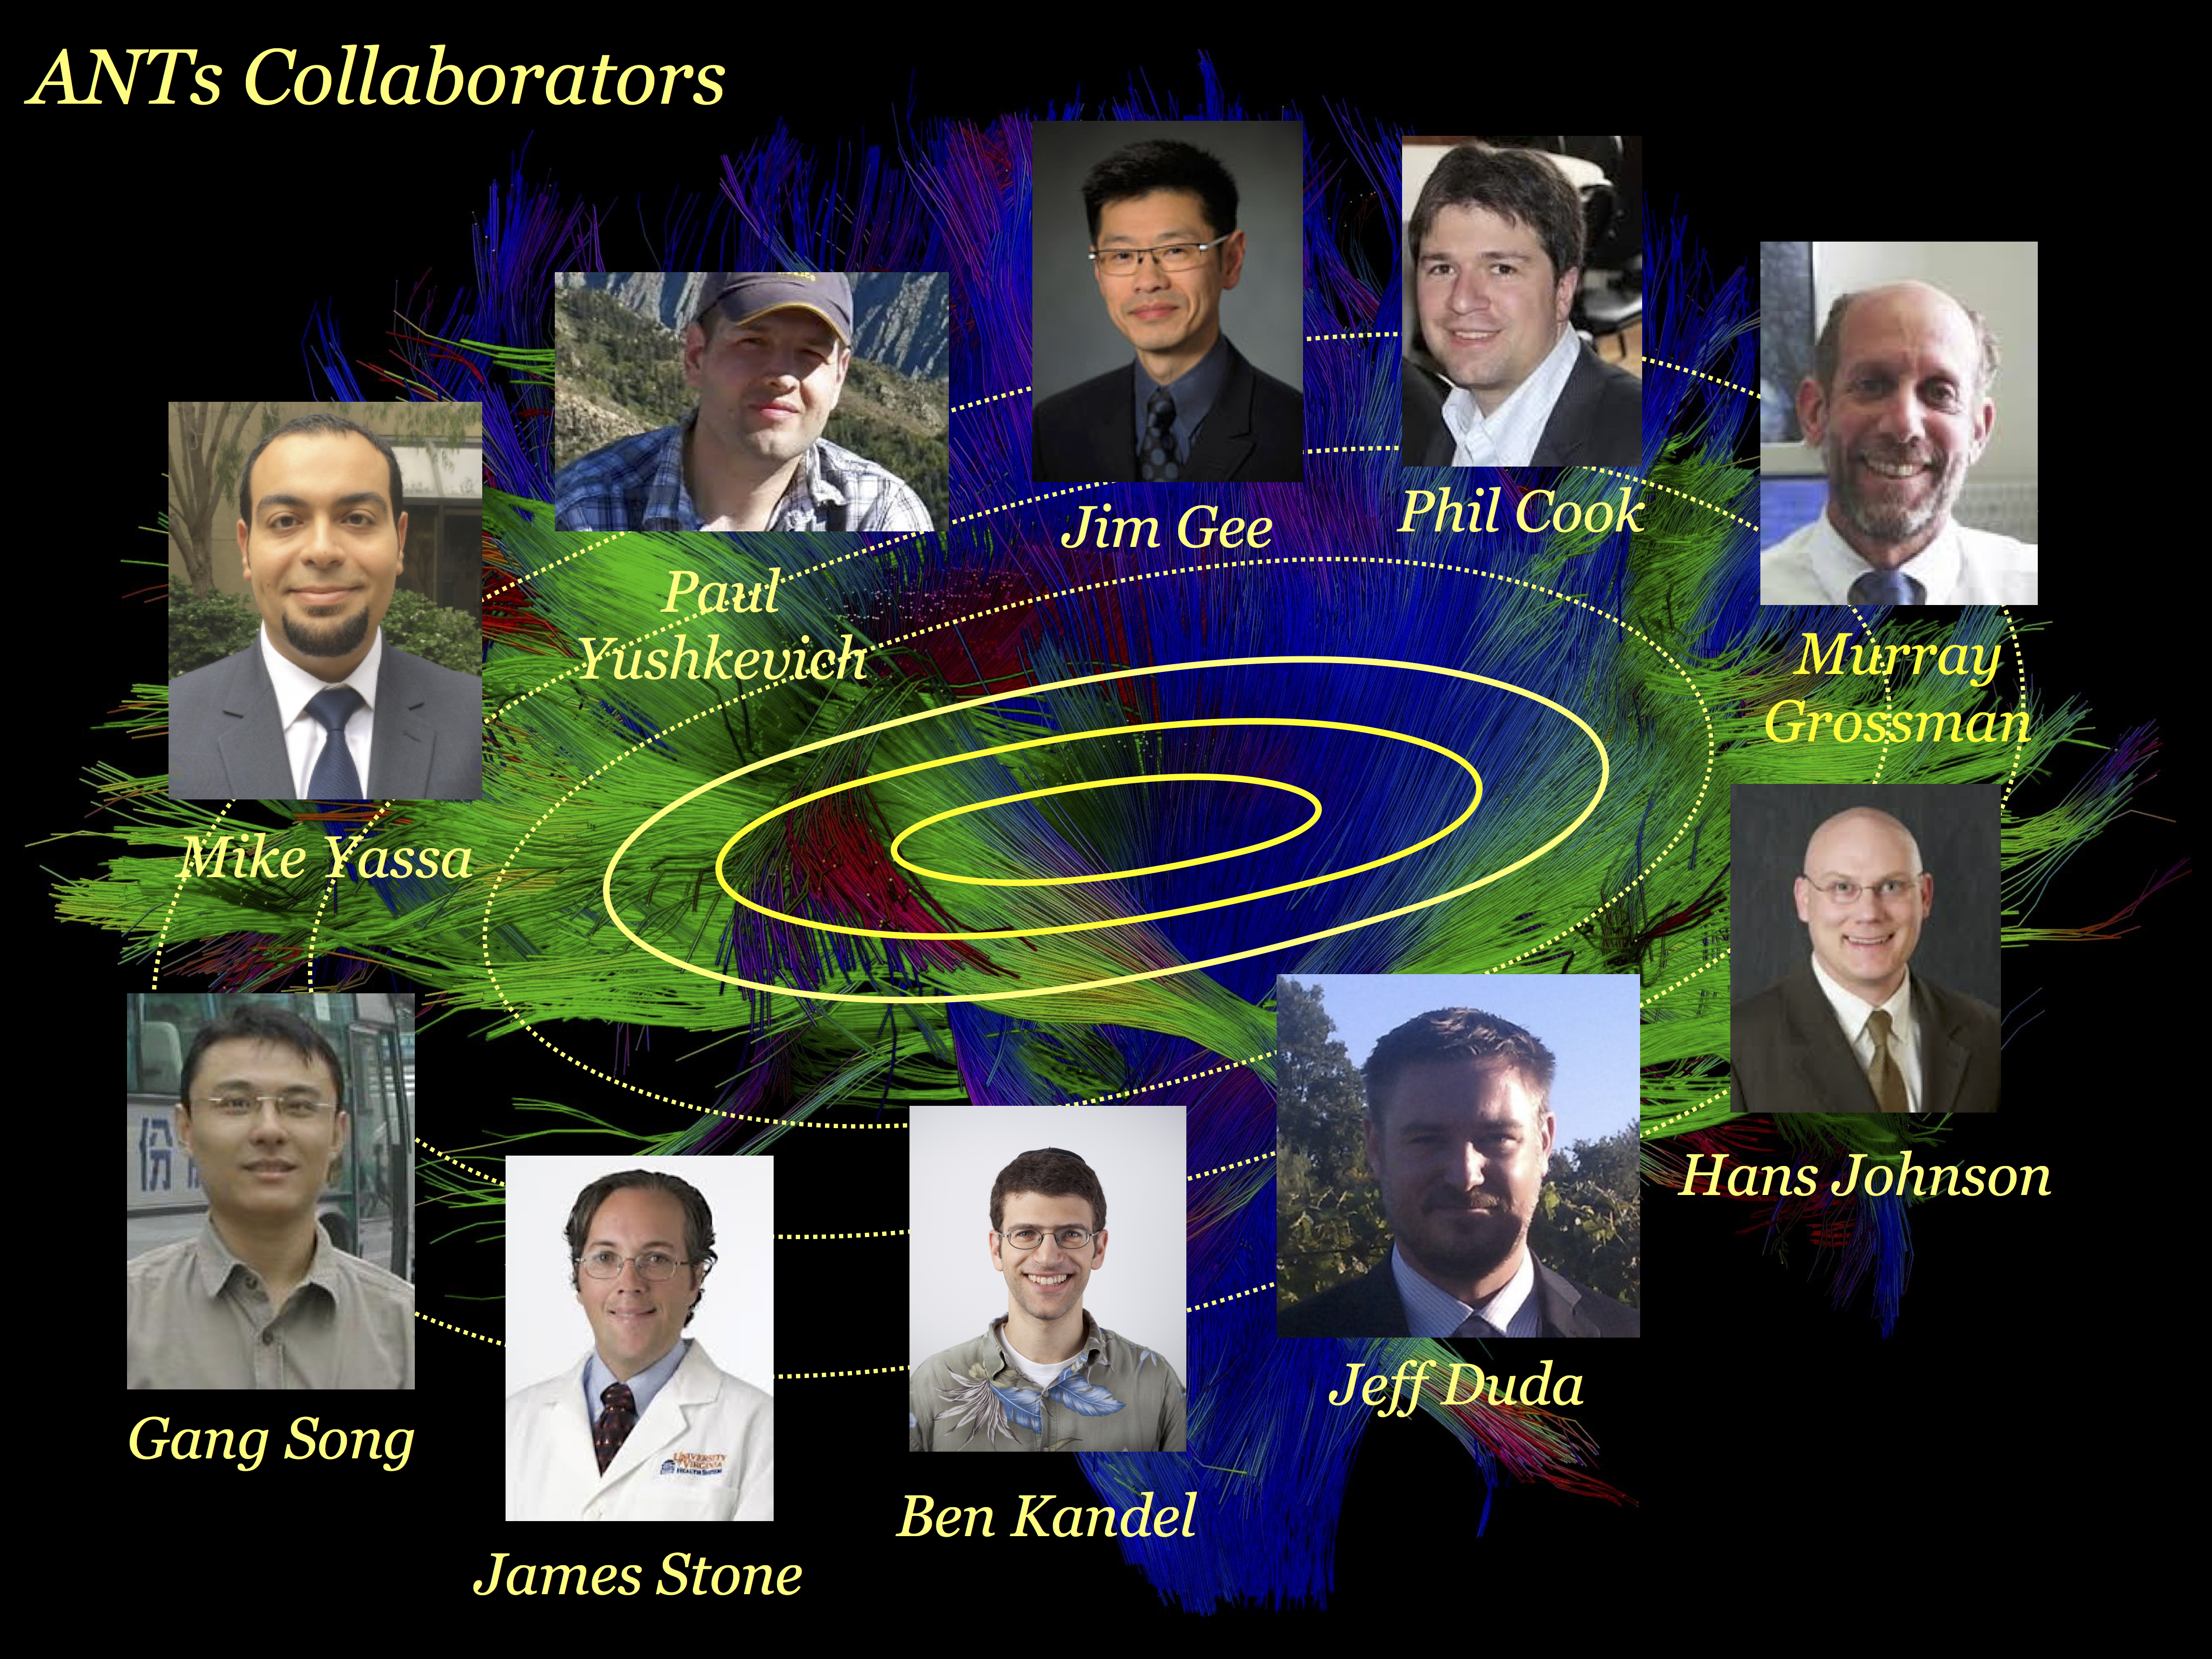
\includegraphics{./figures/antsCollaborators2.png}

\(+\) \href{http://neuro.debian.net/pkgs/ants.html}{neurodebian},
\href{http://www.slicer.org/}{slicer},
\href{https://github.com/BRAINSia/BRAINSTools}{brainsfit},
\href{http://nipy.sourceforge.net/nipype/}{nipype},
\href{http://www.itk.org}{itk} and more \ldots{}

\end{frame}

\section{Why would you care?}\label{why-would-you-care}

\begin{frame}{Software for medical image analysis}

\begin{itemize}
\item
  \href{http://fsl.fmrib.ox.ac.uk/fsldownloads/}{FSL}
\item
  \href{http://www.fil.ion.ucl.ac.uk/spm/software/}{SPM}
\item
  \href{http://www.fil.ion.ucl.ac.uk/spm/software/}{FreeSurfer}
\item
  \href{http://mipav.cit.nih.gov}{MIPAV}
\item
  \href{https://afni.nimh.nih.gov/afni}{AFNI}
\item
  Slicer, Elastix, SimpleITK, ANTs \(\longleftrightarrow\)
  \href{http://www.itk.org}{Insight Toolkit}
\item
  Many more at \href{http://idoimaging.com}{idoimaging.com}
\end{itemize}

\end{frame}

\begin{frame}{International competitions}

\begin{itemize}
\item
  \href{http://www.ncbi.nlm.nih.gov/pubmed/19195496}{Klein 2009}: MRI
  brain registration
\item
  \href{http://empire10.isi.uu.nl}{EMPIRE 2010}: CT lung registration
\item
  \href{https://masi.vuse.vanderbilt.edu/workshop2012/index.php/Main_Page}{Multi-Atlas
  Label Challenge 2012}: MRI brain registration and segmentation
\item
  \href{https://masi.vuse.vanderbilt.edu/workshop2013/index.php/MICCAI_2013_SATA_Challenge_and_Workshop:Current_events}{SATA
  Challenge 2013}: MRI cardiac and canine hind leg registration
\item
  \href{http://martinos.org/qtim/miccai2013/}{BRATS 2013}: Multi-modal
  MRI brain segmentation
\item
  \href{http://www.cardiacatlas.org/web/stacom2014/moco-introduction}{STACOM
  2014 MoCo Challenge}: MRI cardiac motion estimation
\end{itemize}

\end{frame}

\section{Major ANTs utilities}\label{major-ants-utilities}

\begin{frame}{Donoho?}

 \emph{``Papers are just advertisements for the science.''}

\end{frame}

\begin{frame}{Beyond original SyN}

\small

\includegraphics{./papers/figures/Frontiers_ITK.png}

\includegraphics{./papers/figures/Frontiers_BSplineSyN.png}

\end{frame}

\begin{frame}[fragile]{\texttt{antsRegistration}}

\begin{Shaded}
\begin{Highlighting}[]
\NormalTok{$ }\KeywordTok{antsRegistration} \NormalTok{--help}

\KeywordTok{COMMAND}\NormalTok{:}
     \KeywordTok{antsRegistration}
          \KeywordTok{This} \NormalTok{program is a user-level registration application meant to utilize}
          \KeywordTok{ITKv4-only} \NormalTok{classes. The user can specify any number of }\StringTok{"stages"} \NormalTok{where a stage}
          \KeywordTok{consists} \NormalTok{of a transform}\KeywordTok{;} \KeywordTok{an} \NormalTok{image metric}\KeywordTok{;} \KeywordTok{and} \NormalTok{iterations, shrink factors, and}
          \KeywordTok{smoothing} \NormalTok{sigmas for each level.Note that dimensionality, metric, transform,}
          \KeywordTok{output}\NormalTok{, convergence, shrink-factors and smoothing-sigmas parameters are}
          \KeywordTok{mandatory.}

\KeywordTok{OPTIONS}\NormalTok{:}
     \KeywordTok{--version}
          \KeywordTok{Get} \NormalTok{Version Information.}

     \KeywordTok{-d}\NormalTok{, --dimensionality 2/3}
          \KeywordTok{This} \NormalTok{option forces the image to be treated as a specified-dimensional image. If}
          \KeywordTok{not} \NormalTok{specified, we try to infer the dimensionality from the input image.}

     \KeywordTok{-o}\NormalTok{, --output outputTransformPrefix}
                  \NormalTok{[}\KeywordTok{outputTransformPrefix}\NormalTok{,}\KeywordTok{<}\NormalTok{outputWarpedImage}\KeywordTok{>}\NormalTok{,}\KeywordTok{<}\NormalTok{outputInverseWarpedImage}\KeywordTok{>}\NormalTok{]}
          \KeywordTok{Specify} \NormalTok{the output transform prefix (output format is .nii.gz )}\KeywordTok{.} \KeywordTok{Optionally}\NormalTok{, one}
          \KeywordTok{can} \NormalTok{choose to warp the moving image to the fixed space and, if the inverse}
          \KeywordTok{transform} \NormalTok{exists, one can also output the warped fixed image. Note that only the}
          \KeywordTok{images} \NormalTok{specified in the first metric call are warped. Use antsApplyTransforms to}
          \KeywordTok{warp} \NormalTok{other images using the resultant transform(s)}\KeywordTok{.}

     \KeywordTok{-j}\NormalTok{, --save-state saveSateAsTransform}
          \KeywordTok{Specify} \NormalTok{the output file for the current state of the registration. The state}
          \KeywordTok{file} \NormalTok{is written to an hdf5 composite file. It is specially usefull if we want to}
          \KeywordTok{save} \NormalTok{the current state of a SyN registration to the disk, so we can load and}
          \KeywordTok{restore} \NormalTok{that later to continue the next registration process directly started}
          \KeywordTok{from} \NormalTok{the last saved state. The output file of this flag is the same as the}
          \KeywordTok{write-composite-transform}\NormalTok{, unless the last transform is a SyN transform. In that}
          \KeywordTok{case}\NormalTok{, the inverse displacement field of the SyN transform is also added to the}
          \NormalTok{output composite transform. Again notice that this file cannot be treated as a}
          \NormalTok{transform, and restore-state option must be used to load the written file by}
          \NormalTok{this flag.}

     \NormalTok{-k, --restore-state restoreStateAsATransform}
          \NormalTok{Specify the initial state of the registration which get immediately used to}
          \NormalTok{directly initialize the registration process. The flag is mutually exclusive}
          \NormalTok{with other intialization flags.If this flag is used, none of the}
          \NormalTok{initial-moving-transform and initial-fixed-transform cannot be used.}

     \NormalTok{-a, --write-composite-transform 1/(0)}
          \NormalTok{Boolean specifying whether or not the composite transform (and its inverse, if}
          \NormalTok{it exists) should be written to an hdf5 composite file. This is false by default}
          \NormalTok{so that only the transform for each stage is written to file.}
          \NormalTok{<VALUES>: 0}

     \NormalTok{-p, --print-similarity-measure-interval <unsignedIntegerValue>}
          \NormalTok{Prints out the CC similarity metric measure between the full-size input fixed}
          \NormalTok{and the transformed moving images at each iteration a value of 0 (the default)}
          \NormalTok{indicates that the full scale computation should not take placeany value greater}
          \NormalTok{than 0 represents the interval of full scale metric computation.}
          \NormalTok{<VALUES>: 0}

     \NormalTok{-v, --write-interval-volumes <unsignedIntegerValue>}
          \NormalTok{Writes out the output volume at each iteration. It helps to present the}
          \NormalTok{registration process as a short movie a value of 0 (the default) indicates that}
          \NormalTok{this option should not take placeany value greater than 0 represents the}
          \NormalTok{interval between the iterations which outputs are written to the disk.}
          \NormalTok{<VALUES>: 0}

     \NormalTok{-z, --collapse-output-transforms (1)/0}
          \NormalTok{Collapse output transforms. Specifically, enabling this option combines all}
          \NormalTok{adjacent transforms wherepossible. All adjacent linear transforms are written to}
          \NormalTok{disk}\KeywordTok{ in} \NormalTok{the forman itk affine transform }\KeywordTok{(}\NormalTok{called xxxGenericAffine.mat}\KeywordTok{).}
          \KeywordTok{Similarly}\NormalTok{, all adjacent displacement field transforms are combined when written}
          \KeywordTok{to} \NormalTok{disk (e.g. xxxWarp.nii.gz and xxxInverseWarp.nii.gz (if available))}\KeywordTok{.Also}\NormalTok{, an}
          \KeywordTok{output} \NormalTok{composite transform including the collapsed transforms is written to the}
          \KeywordTok{disk} \NormalTok{(called outputCollapsed(Inverse)}\KeywordTok{Composite}\NormalTok{)}\KeywordTok{.}
          \KeywordTok{<VALUES>}\NormalTok{: 1}

     \KeywordTok{-i}\NormalTok{, --initialize-transforms-per-stage (1)}\KeywordTok{/0}
          \KeywordTok{Initialize} \NormalTok{linear transforms from the previous stage. By enabling this option,}
          \KeywordTok{the} \NormalTok{current linear stage transform is directly intialized from the previous}
          \KeywordTok{stage}\StringTok{'s linear transform; this allows multiple linear stages to be run where}
\StringTok{          each stage directly updates the estimated linear transform from the previous}
\StringTok{          stage. (e.g. Translation -> Rigid -> Affine).}
\StringTok{          <VALUES>: 0}

\StringTok{     -n, --interpolation Linear}
\StringTok{                         NearestNeighbor}
\StringTok{                         MultiLabel[<sigma=imageSpacing>,<alpha=4.0>]}
\StringTok{                         Gaussian[<sigma=imageSpacing>,<alpha=1.0>]}
\StringTok{                         BSpline[<order=3>]}
\StringTok{                         CosineWindowedSinc}
\StringTok{                         WelchWindowedSinc}
\StringTok{                         HammingWindowedSinc}
\StringTok{                         LanczosWindowedSinc}
\StringTok{          Several interpolation options are available in ITK. These have all been made}
\StringTok{          available. Currently the interpolator choice is only used to warp (and possibly}
\StringTok{          inverse warp) the final output image(s).}

\StringTok{     -g, --restrict-deformation PxQxR}
\StringTok{          This option allows the user to restrict the optimization of the displacement}
\StringTok{          field, translation, rigid or affine transform on a per-component basis. For}
\StringTok{          example, if one wants to limit the deformation or rotation of 3-D volume to the}
\StringTok{          first two dimensions, this is possible by specifying a weight vector of '}\NormalTok{1x1x0}\StringTok{'}
\StringTok{          for a deformation field or '}\NormalTok{1x1x0x1x1x0}\StringTok{' for a rigid}
\StringTok{          transformation.Low-dimensional restriction only works if there are no preceding}
\StringTok{          transformations.}

\StringTok{     -q, --initial-fixed-transform initialTransform}
\StringTok{                                   [initialTransform,<useInverse>]}
\StringTok{                                   [fixedImage,movingImage,initializationFeature]}
\StringTok{          Specify the initial fixed transform(s) which get immediately incorporated into}
\StringTok{          the composite transform. The order of the transforms is stack-esque in that the}
\StringTok{          last transform specified on the command line is the first to be applied. In}
\StringTok{          addition to initialization with ITK transforms, the user can perform an initial}
\StringTok{          translation alignment by specifying the fixed and moving images and selecting an}
\StringTok{          initialization feature. These features include using the geometric center of the}
\StringTok{          images (=0), the image intensities (=1), or the origin of the images (=2).}

\StringTok{     -r, --initial-moving-transform initialTransform}
\StringTok{                                    [initialTransform,<useInverse>]}
\StringTok{                                    [fixedImage,movingImage,initializationFeature]}
\StringTok{          Specify the initial moving transform(s) which get immediately incorporated into}
\StringTok{          the composite transform. The order of the transforms is stack-esque in that the}
\StringTok{          last transform specified on the command line is the first to be applied. In}
\StringTok{          addition to initialization with ITK transforms, the user can perform an initial}
\StringTok{          translation alignment by specifying the fixed and moving images and selecting an}
\StringTok{          initialization feature. These features include using the geometric center of the}
\StringTok{          images (=0), the image intensities (=1), or the origin of the images (=2).}

\StringTok{     -m, --metric CC[fixedImage,movingImage,metricWeight,radius,<samplingStrategy=\{None,Regular,Random\}>,<samplingPercentage=[0,1]>]}
\StringTok{                  MI[fixedImage,movingImage,metricWeight,numberOfBins,<samplingStrategy=\{None,Regular,Random\}>,<samplingPercentage=[0,1]>]}
\StringTok{                  Mattes[fixedImage,movingImage,metricWeight,numberOfBins,<samplingStrategy=\{None,Regular,Random\}>,<samplingPercentage=[0,1]>]}
\StringTok{                  MeanSquares[fixedImage,movingImage,metricWeight,radius=NA,<samplingStrategy=\{None,Regular,Random\}>,<samplingPercentage=[0,1]>]}
\StringTok{                  Demons[fixedImage,movingImage,metricWeight,radius=NA,<samplingStrategy=\{None,Regular,Random\}>,<samplingPercentage=[0,1]>]}
\StringTok{                  GC[fixedImage,movingImage,metricWeight,radius=NA,<samplingStrategy=\{None,Regular,Random\}>,<samplingPercentage=[0,1]>]}
\StringTok{                  ICP[fixedPointSet,movingPointSet,metricWeight,<samplingPercentage=[0,1]>,<boundaryPointsOnly=0>]}
\StringTok{                  PSE[fixedPointSet,movingPointSet,metricWeight,<samplingPercentage=[0,1]>,<boundaryPointsOnly=0>,<pointSetSigma=1>,<kNeighborhood=50>]}
\StringTok{                  JHCT[fixedPointSet,movingPointSet,metricWeight,<samplingPercentage=[0,1]>,<boundaryPointsOnly=0>,<pointSetSigma=1>,<kNeighborhood=50>,<alpha=1.1>,<useAnisotropicCovariances=1>]}
\StringTok{                  IGDM[fixedImage,movingImage,metricWeight,fixedMask,movingMask,<neighborhoodRadius=0x0>,<intensitySigma=0>,<distanceSigma=0>,<kNeighborhood=1>,<gradientSigma=1>]}
\StringTok{          These image metrics are available--- CC: ANTS neighborhood cross correlation,}
\StringTok{          MI: Mutual information, Demons: (Thirion), MeanSquares, and GC: Global}
\StringTok{          Correlation. The "metricWeight" variable is used to modulate the per stage}
\StringTok{          weighting of the metrics. The metrics can also employ a sampling strategy}
\StringTok{          defined by a sampling percentage. The sampling strategy defaults to '}\NormalTok{None}\StringTok{' (aka}
\StringTok{          a dense sampling of one sample per voxel), otherwise it defines a point set over}
\StringTok{          which to optimize the metric. The point set can be on a regular lattice or a}
\StringTok{          random lattice of points slightly perturbed to minimize aliasing artifacts.}
\StringTok{          samplingPercentage defines the fraction of points to select from the domain. In}
\StringTok{          addition, three point set metrics are available: Euclidean (ICP), Point-set}
\StringTok{          expectation (PSE), and Jensen-Havrda-Charvet-Tsallis (JHCT).}

\StringTok{     -t, --transform Rigid[gradientStep]}
\StringTok{                     Affine[gradientStep]}
\StringTok{                     CompositeAffine[gradientStep]}
\StringTok{                     Similarity[gradientStep]}
\StringTok{                     Translation[gradientStep]}
\StringTok{                     BSpline[gradientStep,meshSizeAtBaseLevel]}
\StringTok{                     GaussianDisplacementField[gradientStep,updateFieldVarianceInVoxelSpace,totalFieldVarianceInVoxelSpace]}
\StringTok{                     BSplineDisplacementField[gradientStep,updateFieldMeshSizeAtBaseLevel,totalFieldMeshSizeAtBaseLevel,<splineOrder=3>]}
\StringTok{                     TimeVaryingVelocityField[gradientStep,numberOfTimeIndices,updateFieldVarianceInVoxelSpace,updateFieldTimeVariance,totalFieldVarianceInVoxelSpace,totalFieldTimeVariance]}
\StringTok{                     TimeVaryingBSplineVelocityField[gradientStep,velocityFieldMeshSize,<numberOfTimePointSamples=4>,<splineOrder=3>]}
\StringTok{                     SyN[gradientStep,updateFieldVarianceInVoxelSpace,totalFieldVarianceInVoxelSpace]}
\StringTok{                     BSplineSyN[gradientStep,updateFieldMeshSizeAtBaseLevel,totalFieldMeshSizeAtBaseLevel,<splineOrder=3>]}
\StringTok{                     Exponential[gradientStep,updateFieldVarianceInVoxelSpace,velocityFieldVarianceInVoxelSpace,<numberOfIntegrationSteps>]}
\StringTok{                     BSplineExponential[gradientStep,updateFieldMeshSizeAtBaseLevel,velocityFieldMeshSizeAtBaseLevel,<numberOfIntegrationSteps>,<splineOrder=3>]}
\StringTok{          Several transform options are available. The gradientStep or learningRate}
\StringTok{          characterizes the gradient descent optimization and is scaled appropriately for}
\StringTok{          each transform using the shift scales estimator. Subsequent parameters are}
\StringTok{          transform-specific and can be determined from the usage. For the B-spline}
\StringTok{          transforms one can also specify the smoothing in terms of spline distance (i.e.}
\StringTok{          knot spacing).}

\StringTok{     -c, --convergence MxNxO}
\StringTok{                       [MxNxO,<convergenceThreshold=1e-6>,<convergenceWindowSize=10>]}
\StringTok{          Convergence is determined from the number of iterations per level and is}
\StringTok{          determined by fitting a line to the normalized energy profile of the last N}
\StringTok{          iterations (where N is specified by the window size) and determining the slope}
\StringTok{          which is then compared with the convergence threshold.}

\StringTok{     -s, --smoothing-sigmas MxNxO...}
\StringTok{          Specify the sigma of gaussian smoothing at each level. Units are given in terms}
\StringTok{          of voxels ('}\NormalTok{vox}\StringTok{') or physical spacing ('}\NormalTok{mm}\StringTok{'). Example usage is '}\NormalTok{4x2x1mm}\StringTok{' and}
\StringTok{          '}\NormalTok{4x2x1vox}\StringTok{' where no units implies voxel spacing.}

\StringTok{     -f, --shrink-factors MxNxO...}
\StringTok{          Specify the shrink factor for the virtual domain (typically the fixed image) at}
\StringTok{          each level.}

\StringTok{     -u, --use-histogram-matching}
\StringTok{          Histogram match the images before registration.}

\StringTok{     -l, --use-estimate-learning-rate-once}
\StringTok{          turn on the option that lets you estimate the learning rate step size only at}
\StringTok{          the beginning of each level. * useful as a second stage of fine-scale}
\StringTok{          registration.}

\StringTok{     -w, --winsorize-image-intensities [lowerQuantile,upperQuantile]}
\StringTok{          Winsorize data based on specified quantiles.}

\StringTok{     -x, --masks [fixedImageMask,movingImageMask]}
\StringTok{          Image masks to limit voxels considered by the metric.}

\StringTok{     --float}
\StringTok{          Use '}\NormalTok{float}\StringTok{' instead of '}\NormalTok{double}\StringTok{' for computations.}
\StringTok{          <VALUES>: 0}

\StringTok{     -v, --verbose (0)/1}
\StringTok{          Verbose output.}

\StringTok{     -h}
\StringTok{          Print the help menu (short version).}

\StringTok{     --help}
\StringTok{          Print the help menu. Will also print values used on the current command line}
\StringTok{          call.}
\end{Highlighting}
\end{Shaded}

\end{frame}

\begin{frame}{Template building: creating the average Joe}

\includegraphics{./papers/figures/template0.jpg}

\end{frame}

\begin{frame}{``Attractiveness'' \(\rightarrow\) mental processing?}

\includegraphics{./papers/figures/template1.jpg}

\end{frame}

\begin{frame}{What about brains?}

\includegraphics{./papers/figures/template3.jpg}

\end{frame}

\begin{frame}{Templates facilitate computation}

\includegraphics{./papers/figures/template4.jpg}

\end{frame}

\begin{frame}{Gender discernibility?}

\includegraphics{./papers/figures/template5.jpg}

\end{frame}

\begin{frame}{Nonparametric nonuniform intensity normalization (N3)}

\begin{itemize}
\item
  Developed at the Montreal Neurological Institute (John Sled, 1998)
\item
  Part of the standard preprocessing protocol in large scale projects
  such as ADNI
\item
  The traditional de facto standard in MRI bias correction

  \begin{itemize}
  \tightlist
  \item
    good performance
  \item
    \emph{public availability}
  \end{itemize}
\item
  Public availability --- set of perl scripts coordinating various C++
  programs
\item
  ``\emph{Let's incorporate N3 into ANTs!}''
\end{itemize}

\end{frame}

\begin{frame}{N3 adoption issues}

\includegraphics{./tools/n4/figures/whyN4.png}

\end{frame}

\begin{frame}{Atropos: flexible code base}

``20+ years of development. \emph{Show me the code!}''

\includegraphics{./tools/atropos/figures/atropos.png}

\end{frame}

\begin{frame}{Atropos + N4 \(\rightarrow\) \texttt{antsAtroposN4.sh}}

\includegraphics{./tools/atropos/figures/atroposFlow.png}

\end{frame}

\begin{frame}{\texttt{DenoiseImage} --- contribution from Jose Manjon}

\includegraphics{./tools/figures/denoising.png}

\end{frame}

\begin{frame}{Multi-atlas segmentation}

\includegraphics{./tools/jointfusion/figures/jointLabelFusion.png}

\end{frame}

\begin{frame}{New work: joint intensity fusion}

\includegraphics{./tools/jointfusion/figures/jointIntensityFusion.png}

\end{frame}

\begin{frame}{Possible uses}

\begin{itemize}
\item
  ``Correct'' images

  \begin{itemize}
  \item
    motion correction
  \item
    ``remove'' lesions
  \end{itemize}
\item
  Project atlas set intensity signature
\item
  Use in ``corrective learning''
\end{itemize}

\end{frame}

\section{Putting it all together---the ANTs cortical thickness
pipeline}\label{putting-it-all-togetherthe-ants-cortical-thickness-pipeline}

\begin{frame}{Cortical thickness studies}

\begin{longtable}[c]{@{}ll@{}}
\toprule
Column1 & Column2\tabularnewline
\midrule
\endhead
Tetris-playing ability & chronic pancreatitis\tabularnewline
Huntington's disease & obsessive-compulsive disorder\tabularnewline
schizophrenia & ADHD\tabularnewline
bipolar disorder & obesity\tabularnewline
Alzheimer's disease & heritable depression\tabularnewline
frontotemporal dementia & elderly depression\tabularnewline
Parkinson's disease & age\tabularnewline
Williams syndrome & gender\tabularnewline
multiple sclerosis & handedness\tabularnewline
autism & intelligence\tabularnewline
migraines & athletic ability\tabularnewline
chronic smoking & meditative practices\tabularnewline
alcoholism & musical ability\tabularnewline
cocaine addiction & tendency toward criminality\tabularnewline
Tourette syndrome in children & childhood sexual abuse in female
adolescents\tabularnewline
scoliosis in female adolescents & traumatic brain injury\tabularnewline
early-onset blindness & untreated male-to-female
transsexuality\tabularnewline
\bottomrule
\end{longtable}

\end{frame}

\begin{frame}{The ANTs structural brain mapping workflow}

\includegraphics{./evaluation/figures/pipeline.png}

\end{frame}

\begin{frame}{Template building}

\emph{Tailor data to your specific cohort}

\includegraphics{./evaluation/figures/templates.png}

\end{frame}

\begin{frame}{Template priors}

\includegraphics{./evaluation/figures/templatePriors.png}

\end{frame}

\begin{frame}{Cortical thickness maps}

\includegraphics{./evaluation/figures/corticalThicknessEstimation.png}

In contrast to FreeSurfer which warps coupled surface meshes to segment
the gray matter, \emph{ANTs} diffeomorphically registers the white
matter to the combined gray/white matters while simultaneously
estimating thickness.

\end{frame}

\begin{frame}

\emph{But without ground truth, how does one evaluate the pipeline?}

\end{frame}

\begin{frame}{Predict age and gender}

\(AGE \sim VOLUME + GENDER + \sum_{i=1}^{62} T(DKT_i)\)

\end{frame}

\begin{frame}{Prediction from cortical thickness data}

\includegraphics{./evaluation/figures/evaluation.png}

\end{frame}

\begin{frame}{Age prediction per site}

\includegraphics{./evaluation/figures/agePredictionPerSite.png}

\end{frame}

\begin{frame}{Regional importance comparison}

\includegraphics{./evaluation/figures/antsvfreesurfer_Importance.png}

ANTs (left) vs.~FreeSurfer (right)

\end{frame}

\begin{frame}{Regional measurements}

\includegraphics{./evaluation/figures/antsvfreesurfer_regionalPlots.png}

\end{frame}

\section{But, wait, there's more!}\label{but-wait-theres-more}

\begin{frame}{ANTs tools are multivariate}

\includegraphics{./evaluation/figures/rfRmse05ANTsT1T2.png}

\end{frame}

\begin{frame}{Longitudinal processing}

\includegraphics{./longitudinal/figures/longitudinalPipeline.png}

\end{frame}

\section{Current work and Advanced Normalization Tools in R
(ANTsR)}\label{current-work-and-advanced-normalization-tools-in-r-antsr}

\begin{frame}{Multimodal Brain Tumor Segmentation (BRATS 2013)}

\includegraphics{./competitions/figures/brats2013results2.png}

\href{http://www.ncbi.nlm.nih.gov/pubmed/25433513}{Tustison, et al.,
Optimal symmetric multimodal templates and concatenated random forests
for supervised brain tumor segmentation (simplified) with \emph{ANTsR},
\emph{Neuroinformatics}.}

\end{frame}

\begin{frame}{White matter hyperintensities in TBI}

\includegraphics{./wmhs/figures/wmhPipeline.png}

\end{frame}

\begin{frame}{Social behavior and immunity dysfunction in mice}

\includegraphics{./antsr/figures/filiano_rsfmri.png}

\end{frame}

\begin{frame}{Other ANTsR work}

\begin{itemize}
\item
  \href{http://www.nature.com/articles/sdata20153}{Pediatric template of
  brain perfusion}
\item
  \href{http://www.ncbi.nlm.nih.gov/pubmed/26756101}{Automated
  segmentation of chronic stroke lesions using LINDA: Lesion
  identification with neighborhood data analysis}
\item
  \href{http://www.ncbi.nlm.nih.gov/pubmed/25448483}{Eigenanatomy}
\item
  Corrective learning for segmentation refinement
\end{itemize}

\hypertarget{refs}{}

\end{frame}

\end{document}
